\documentclass[12pt]{article}
\usepackage{graphicx, color}
\usepackage[utf8]{inputenc}
\usepackage{amsfonts}
\usepackage{amsmath}
\usepackage[T1]{fontenc}
\usepackage{xcolor}
\usepackage{float}
\usepackage{textcomp}
\usepackage{multicol}
\usepackage[portuges]{babel}
\usepackage{xcolor}
\usepackage[round]{natbib}
\usepackage[utf8]{inputenc}
\usepackage{amsmath,amssymb}
\usepackage{hyperref}
\usepackage{longtable}
\usepackage{subfig}
\usepackage{soul}
\usepackage{booktabs}

\vfuzz2pt
\hfuzz2pt
\newtheorem{thm}{Theorem}[section]
\newtheorem{cor}[thm]{Corollary}
\newtheorem{lem}[thm]{Lemma}
\newtheorem{prop}[thm]{Proposition}
\newtheorem{defn}[thm]{Definition}
\newtheorem{rem}[thm]{Remark}
\numberwithin{equation}{section}
\newcommand{\norm}[1]{\left\Vert#1\right\Vert}
\newcommand{\abs}[1]{\left\vert#1\right\vert}
\newcommand{\set}[1]{\left\{#1\right\}}
\newcommand{\Real}{\mathbb R}
\newcommand{\eps}{\varepsilon}
\newcommand{\To}{\longrightarrow}
\newcommand{\BX}{\mathbf{B}(X)}
\newcommand{\A}{\mathcal{A}}
\usepackage{anysize}
\usepackage[left=2.0cm,top=2.5cm,right=1.5cm,bottom=2.0cm]{geometry}

\renewcommand*\contentsname{Conteúdo}

\begin{document}
\thispagestyle{empty}

%%%%%%%%%%%%%%%%%%%%%%%%%%%%%%%%%%%%%%%%%%%%%%%%%%%%%%%%%%%%%%%%%%%%%%%%%%%%%%%%%%%%%%%%%%
%%%%%%%             CAPA DO TRABALHO ou Folha de rosto                       %%%%%%%%%%%%
%%%%%%%%%%%%%%%%%%%%%%%%%%%%%%%%%%%%%%%%%%%%%%%%%%%%%%%%%%%%%%%%%%%%%%%%%%%%%%%%%%%%%%%%%%

\begin{figure}
  \centering
  
\includegraphics[scale=0.5]{logoon.png}
  \vspace*{-0.3cm}
\end{figure}

\begin{center}
{\large \rm \textbf {OBSERVATÓRIO NACIONAL} \linebreak}
{\large \rm \textbf {MINISTÉRIO DA CIÊNCIA E TECNOLOGIA} \linebreak}
{\large \rm \textbf {PROGRAMA DE PÓS-GRADUAÇÃO EM ASTRONOMIA} \linebreak}
\end{center}

\baselineskip 30pt

\vspace*{0.3cm}

\begin{center}
{\LARGE \bfseries Relatório de Atividades \\ (2º Relatório)}
\end{center}

\vspace*{1cm}

\setcounter{footnote}{1}

\renewcommand{\thefootnote}{\fnsymbol{footnote}}
\begin{center}
{\sc  Aluno: Thiago Laidler Vidal Cunha

\vspace*{0.3cm}

{\sc  Orientador: Julio Ignacio Bueno de Camargo
\\}

\end{center}

\setcounter{footnote}{1}

\vspace*{2.8cm}

\begin{flushleft}
Início do Mestrado: Março de 2024\\
Bolsa: Sem bolsa\\
Período coberto: Agosto de 2025 -- Abril de 2026\\
\end{flushleft}

\baselineskip 17pt

\vspace*{1.5cm}
\begin{center}
{{\bf Rio de Janeiro\par{Abril de 2026}}}
\end{center}

\vspace*{.05cm}

\renewcommand{\thefootnote}{\arabic{footnote}}

\setcounter{footnote}{1}

\pagebreak

\baselineskip 19pt

%%%%%%%%%%%%%%%%%%%%%%%%%%%%%%%%%   SUMÁRIO   %%%%%%%%%%%%%%%%%%%%%%%%%%%%%%%%%%%%%%%%%%%%%%%%%

\pagenumbering{roman}
\pagestyle{fancy}
\tableofcontents
\pagenumbering{arabic}

%*****************************************************************
%PROJETO
%*****************************************************************

\newpage

\section{\sc Projeto}

O projeto de mestrado intitulado \textit{``Pipeline para Detecção Automatizada de Ocultações Estelares em Curvas de Luz com Técnicas de Machine Learning''} chega a esta segunda etapa de relatório com a maior parte de seus objetivos científicos cumpridos: a \textit{pipeline} foi inteiramente implementada, validada experimentalmente e a dissertação encontra-se em revisão final, com defesa prevista para o segundo semestre de 2026.

A motivação original permanece: ocultações estelares -- eventos em que um corpo do Sistema Solar passa diante de uma estrela distante, bloqueando sua luz -- são uma das técnicas mais precisas para a determinação de dimensões e formas projetadas de asteroides, Centauros e Objetos Transnetunianos (TNOs), com resolução comparável à de sondas espaciais \citep{Sicardy2011, Knieling2024}. O crescimento contínuo do volume de dados produzido por redes de telescópios profissionais e amadores, somado à melhoria astrométrica do catálogo Gaia, tornou a triagem manual de todas as curvas custosa e impulsionou a adoção de métodos automatizados. Esta dissertação responde a essa demanda com uma \textit{pipeline} interpretável, baseada em \textit{features} clássicas extraídas das séries temporais e classificadores de árvore.

Em relação ao primeiro relatório, o projeto evoluiu em todas as frentes previstas: o conjunto de dados foi consolidado e ampliado; as características numéricas foram formalizadas e racionalizadas por análise de redundância; quatro classificadores foram treinados, comparados e auditados em sete experimentos sucessivos; um simulador físico de curvas de luz foi incorporado para gerar negativos sintéticos; e uma análise de ajuste de limiar foi desenvolvida para permitir operação em regime de alta sensibilidade. Os resultados obtidos -- F1-score entre 0,978 e 0,994 e AUC-ROC superior a 0,998 no conjunto de teste -- corroboram a hipótese formulada no primeiro relatório.

\subsection{Objetivo Científico}

Os objetivos principais do projeto, conforme estabelecidos no primeiro relatório, foram:

\begin{itemize}
    \item Organizar e disponibilizar um banco de curvas de luz estruturado, servindo como recurso para futuras pesquisas em ocultações estelares;
    \item Desenvolver uma ferramenta automatizada de classificação, capaz de identificar quais curvas apresentam ocultações reais, auxiliando astrônomos na triagem e análise dos dados.
\end{itemize}

Ambos os objetivos foram atingidos. O banco de dados relacional em SQLite contém atualmente 1693 curvas de luz catalogadas, das quais 802 são positivas reais (provenientes do catálogo \texttt{B/occ/asteroid} do VizieR e do banco do Grupo do Rio), 186 são negativos artificiais obtidos por recorte manual de segmentos sem ocultação a partir de curvas positivas, 3 são negativas reais e 702 são curvas sintéticas geradas pelo simulador físico de \cite{Simulator}. A \textit{pipeline} de classificação foi implementada em Python e está documentada para reprodução.

\subsection{Resumo dos Resultados}

O sistema desenvolvido demonstra, em sete experimentos sucessivos com diferentes configurações de \textit{features} e divisões treino/teste, que classificadores tradicionais (Regressão Logística, Random Forest, XGBoost e CatBoost) com \textit{features} fisicamente motivadas atingem desempenho comparável ou superior a abordagens baseadas em redes convolucionais reportadas na literatura \citep{Cazeneuve_2023}, com a vantagem adicional de interpretabilidade. Um estudo de ablação evidenciou que a \textit{feature} apontada como mais importante pelos modelos de árvore (distância entre centróides do K-Means) é, na prática, dispensável -- resultado relevante, pois mostra que importância algorítmica não implica insubstituibilidade. Uma análise complementar de ajuste do limiar de decisão demonstrou que a \textit{pipeline} pode operar em regime de alta sensibilidade (minimização de falsos negativos) em pós-processamento, sem necessidade de retreinamento -- estratégia adequada à triagem científica, em que o custo de perder um evento genuíno supera o de revisar um alarme falso.

\section{\sc Informações curriculares}

\subsection{Disciplinas Cursadas}

{\small
\begin{tabular}{|c|l|c|c|}
\hline
Ano/Semestre & Disciplina & Conceito & Créditos \\
\hline
2024/1       & Astronomia de Posição    & A & 4  \\
2024/1       & Evolução Estelar	& A & 4  \\
2024/2       & Astroestatística         & A & 4  \\
2024/1       & Astronomia Dinâmica      & A & 4  \\
2024/2       & Tópicos de E-Science     & A & 4  \\
2024/2       & Propriedades Físicas de Pequenos Corpos & A & 4 \\
\hline
\hline
\end{tabular}
}

\subsection{Atividades}

\begin{itemize}
    \item Coautoria no artigo \cite{Umbriel2020}, referente à campanha de ocultação de Umbriel observada em 2020.
    \item Continuidade do desenvolvimento da \textit{pipeline} em Python, com versionamento em repositório Git e documentação completa para reprodução.
\end{itemize}

\subsection{Exame de Proficiência}

Aprovado no exame de proficiência oferecido pelo Observatório Nacional em 2024.

%%%%%%%%%%%%%%%%%%%%%%%%%%%%%%%%%%%%%%%%%%%%%%%%%%%%%%%%%%%%%%%%%%%%%%%%%%%%%%%%%%%%%
%%%%%%%     Capitulo: Situação à época do último relatório                  %%%%%%%%
%%%%%%%%%%%%%%%%%%%%%%%%%%%%%%%%%%%%%%%%%%%%%%%%%%%%%%%%%%%%%%%%%%%%%%%%%%%%%%%%%%%%%

\section{Situação do projeto à época do último relatório}

No primeiro relatório (agosto de 2025), o projeto encontrava-se na seguinte situação:

\begin{itemize}
    \item \textbf{Banco de dados:} já consolidado em SQLite, com 931 curvas obtidas do VizieR e curvas adicionais do Grupo do Rio (Umbriel 2020 e Chiron 2023). A arquitetura relacional, com tabelas \texttt{observations} e \texttt{light\_curves}, encontrava-se estável.

    \item \textbf{Pré-processamento:} \textit{scripts} de aquisição assíncrona via \texttt{astroquery}/\texttt{aiohttp} e de inserção no banco já estavam em funcionamento.

    \item \textbf{Engenharia de \textit{features}:} encontrava-se em fase inicial. Eram extraídas estatísticas básicas (média, desvio padrão, mínimo, máximo, médias por quartil), com mais grandezas em estudo.

    \item \textbf{Balanceamento do \textit{dataset}:} a desproporção entre positivas (mais de 90\%) e negativas havia sido identificada como problema; o recorte manual de segmentos sem ocultação a partir de curvas positivas estava em curso, e a geração de curvas sintéticas via simulador de \cite{Simulator} estava prevista, mas ainda não implementada.

    \item \textbf{Treinamento:} ainda não iniciado. Os modelos planejados (XGBoost e Random Forest) haviam sido escolhidos, mas nenhuma classificação havia sido produzida.

    \item \textbf{Dissertação:} escrita iniciada, com estrutura definida.
\end{itemize}

Todas as etapas previstas naquele relatório foram concluídas. As próximas seções detalham os avanços do período 2025-08 a 2026-04.

%%%%%%%%%%%%%%%%%%%%%%%%%%%%%%%%%   PESQUISA DETALHADA   %%%%%%%%%%%%%%%%%%%%%%%%%%%%%%%%%%%%%

\section{\sc Descrição detalhada da pesquisa}

\subsection{Arquitetura final da \textit{pipeline}}\label{sec_arquitetura}

A metodologia consolidou-se em uma \textit{pipeline} de cinco etapas sucessivas, na qual a saída de um bloco alimenta o seguinte. A Figura~\ref{fig:diagrama_pipeline} ilustra o fluxo completo, desde as fontes de dados até os modelos treinados.

\begin{figure}[!h]
\begin{center}
    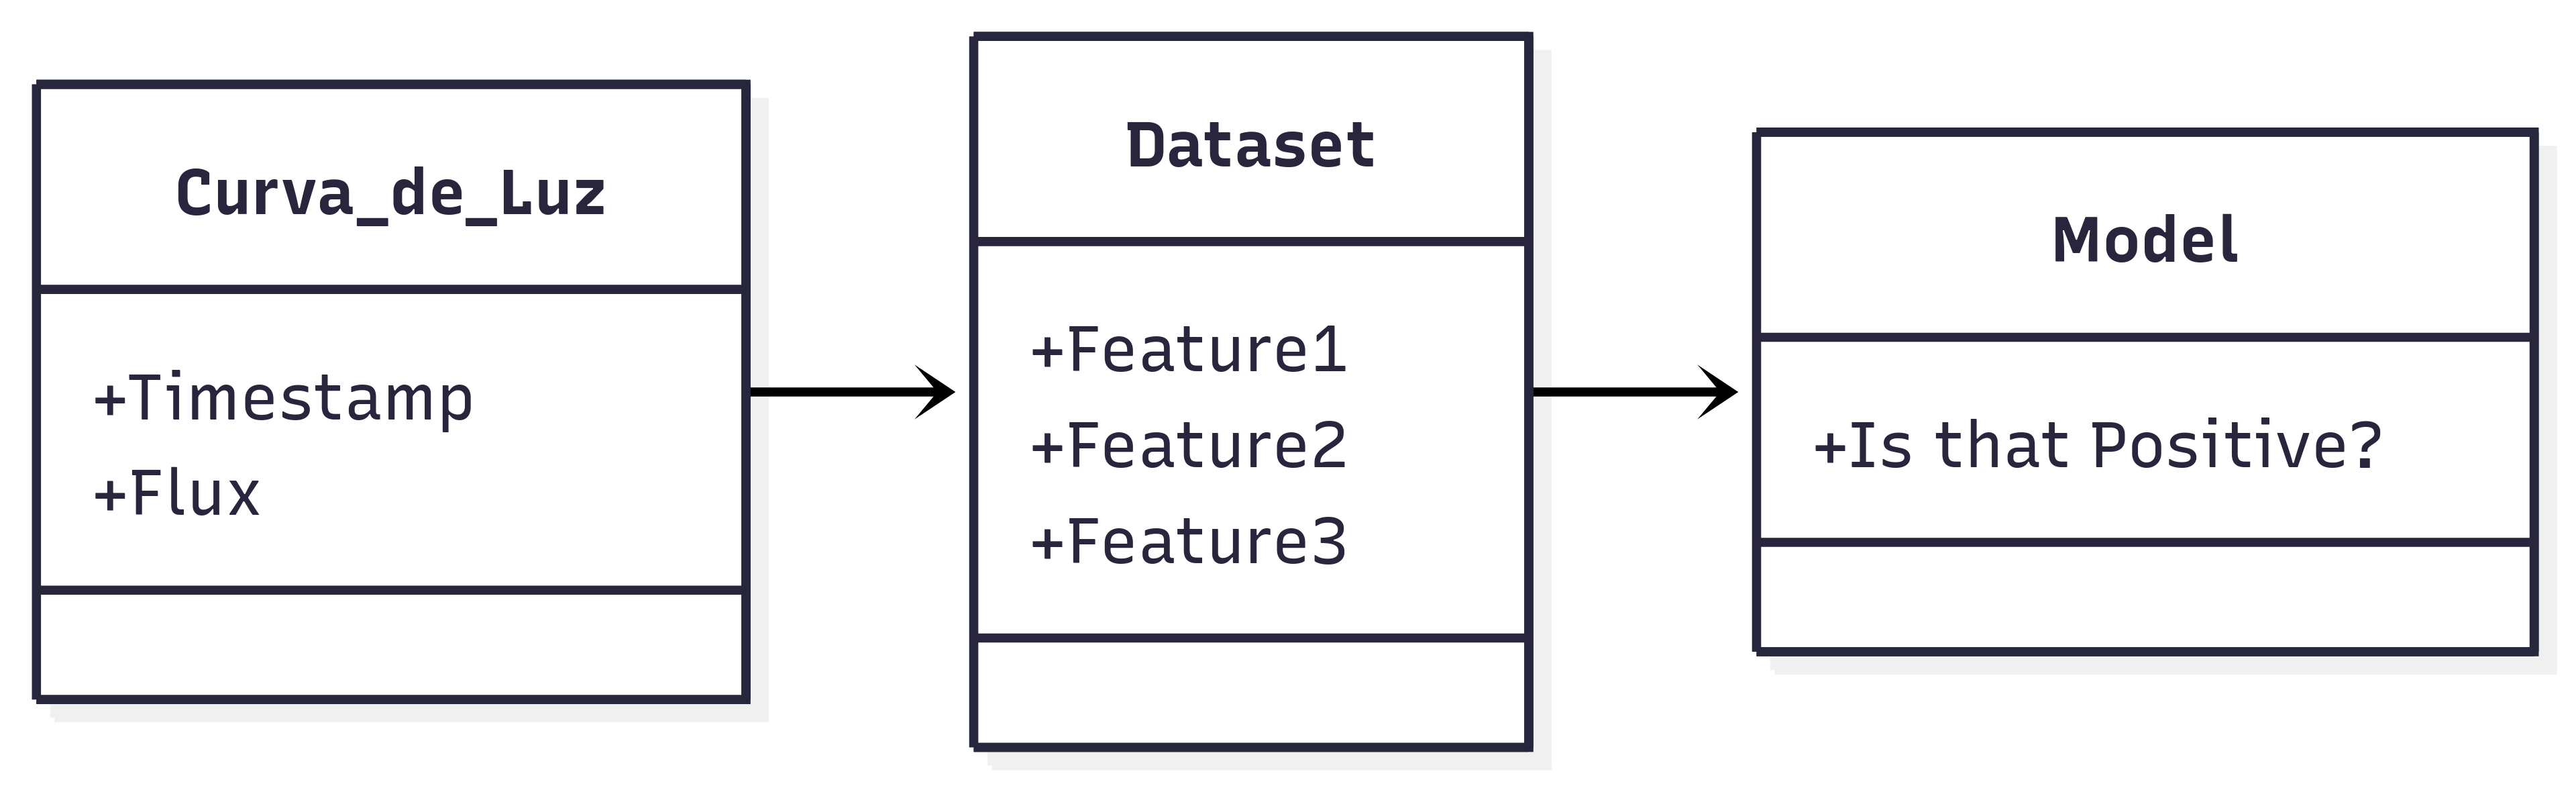
\includegraphics[scale=0.08]{diagrama_1.png}
\caption{Esquema da \textit{pipeline}: as curvas de luz são convertidas em vetores de \textit{features} antes do treinamento; os classificadores operam sobre essas \textit{features}, e não sobre as séries temporais brutas.}
\label{fig:diagrama_pipeline}
\end{center}
\end{figure}

\textbf{Etapa 1 -- Aquisição e armazenamento.} Curvas de luz são obtidas a partir do catálogo \texttt{B/occ/asteroid} do VizieR (agregador público que reúne campanhas independentes envolvendo múltiplos observadores, telescópios e corpos) e do banco em nuvem do Grupo do Rio (campanhas específicas de Umbriel \citep{Umbriel2020} e Chiron \citep{Chiron2023}). Os dados são inseridos no banco SQLite (\texttt{observations} e \texttt{light\_curves}), com integridade referencial garantida. A arquitetura é genérica: novos catálogos podem ser incorporados mediante adaptador de metadados específico, sem alteração no restante do sistema.

\textbf{Etapa 2 -- Acesso e normalização.} Um módulo dedicado consulta o banco, filtra curvas por critérios (objeto, data, tipo) e aplica a normalização do fluxo. A estratégia adotada divide a série temporal em quatro segmentos contíguos (quartis temporais), seleciona as duas médias mais altas como representativas do nível fora da ocultação e usa sua média como \textit{baseline}. O fluxo é então dividido por esse \textit{baseline}, fazendo com que curvas sem evento permaneçam próximas de 1 e curvas com evento exibam quedas abaixo de 1.

\textbf{Etapa 3 -- Construção do conjunto de dados.} As curvas disponíveis são reunidas; segmentos sem ocultação são recortados manualmente de curvas positivas (com revisão humana e exclusão da positiva original do conjunto de treino para evitar vazamento); curvas sintéticas negativas geradas pelo simulador físico de \cite{Simulator} são incorporadas. O \textit{dataset} final reúne 1693 amostras (Tabela~\ref{tab:dataset_fonte}).

\begin{table}[!h]
\centering
\caption{Composição do \textit{dataset} utilizado nos experimentos.}
\label{tab:dataset_fonte}
\begin{tabular}{lc}
\toprule
\textbf{Fonte} & \textbf{Quantidade} \\
\midrule
Curvas positivas do banco (VizieR + Grupo do Rio) & 802 \\
Negativos artificiais (recorte manual de positivas) & 186 \\
Curvas negativas do banco & 3 \\
Curvas sintéticas negativas (simulador físico) & 702 \\
\midrule
\textbf{Total} & \textbf{1693} \\
\bottomrule
\end{tabular}
\end{table}

\textbf{Etapa 4 -- Extração de \textit{features}.} Cada curva é convertida em um vetor numérico que descreve estatísticas do fluxo, características derivadas de suavização (média móvel e Savitzky-Golay), \textit{max drawdown}, distância entre centróides do K-Means aplicado ao fluxo suavizado, testes estatísticos entre quartis temporais (teste $t$ de Welch e Kolmogorov-Smirnov) e métricas observacionais inspiradas na análise de ocultações (profundidade do \textit{dip}, SNR do \textit{dip}, duração do maior bloco abaixo do \textit{baseline}, $\chi^2$ de modelos constante e \textit{square well}, e a razão entre eles). O conjunto inicial continha 28 \textit{features}; uma análise de redundância (correlações altas, derivações algébricas, variância desprezível) reduziu o conjunto a 13 variáveis sem perda de desempenho.

\textbf{Etapa 5 -- Treinamento e avaliação.} Quatro classificadores são treinados: Regressão Logística (com regularização $\ell_2$), Random Forest, XGBoost e CatBoost. A divisão treino/teste é estratificada por curva (cada curva aparece integralmente em treino \emph{ou} teste, nunca nos dois) com sementes fixas para reprodutibilidade. As características são padronizadas (\texttt{StandardScaler}) apenas para a Regressão Logística; os modelos baseados em árvores recebem as variáveis em escala original. As métricas reportadas são acurácia, precisão, sensibilidade, F1-score e AUC-ROC, sempre no conjunto de teste.

\subsection{Modelos e algoritmos}

A escolha dos quatro classificadores foi orientada pelo princípio de \textbf{interpretabilidade} aliada a desempenho competitivo:

\begin{itemize}
    \item \textbf{Regressão Logística:} classificador linear probabilístico, ajustado por gradiente descendente sobre a função de custo de entropia cruzada. Serve como \textit{baseline} interpretável.

    \item \textbf{Random Forest:} \textit{ensemble} de árvores treinadas em amostras \textit{bootstrap} dos dados; a aleatoriedade na escolha de \textit{features} em cada nó descorrelaciona as árvores e reduz a variância. O Teorema do Júri de Condorcet sustenta a intuição: árvores com acurácia individual de 65\% podem produzir um \textit{ensemble} com acurácia próxima de 94\% (Figura~\ref{fig:condorcet}).

    \item \textbf{XGBoost:} \textit{gradient boosting} com regularização explícita e expansão de Taylor de segunda ordem da perda; árvores treinadas sequencialmente para corrigir erros do modelo anterior.

    \item \textbf{CatBoost:} também \textit{gradient boosting}, com \textit{ordered boosting} (mitigação de \textit{target leakage}) e árvores \textit{oblivious} (regularização estrutural).
\end{itemize}

\begin{figure}[!h]
\begin{center}
    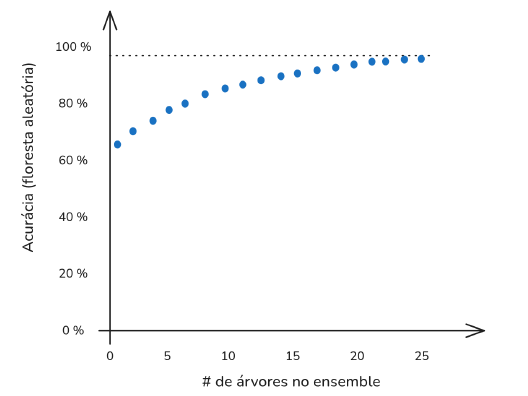
\includegraphics[scale=0.55]{manual_2.png}
\caption{Ilustração do Teorema do Júri de Condorcet aplicado a \textit{ensembles}: 25 árvores com acurácia individual em torno de 65\% podem resultar em uma floresta com acurácia próxima de 94\%, desde que os erros não sejam idênticos.}
\label{fig:condorcet}
\end{center}
\end{figure}

A escolha do limiar de decisão (\textit{threshold} $\tau$) foi tratada como hiperparâmetro de pós-processamento. Embora $\tau = 0{,}5$ seja o valor padrão, sua redução para $\tau \approx 0{,}1$--$0{,}3$ permite operar em regime de alta sensibilidade sem retreinamento, conforme demonstrado no Capítulo 5 da dissertação.

\subsection{Validação por \textit{k-fold} estratificado}

Além da divisão treino/teste única, foi implementada validação cruzada estratificada por curva (Figura~\ref{fig:kfold}), garantindo que cada curva apareça apenas em uma das dobras. Essa estratégia fornece estimativas mais robustas do erro de generalização, permitindo reportar média e desvio padrão das métricas em vez de um valor único.

\begin{figure}[!h]
\begin{center}
    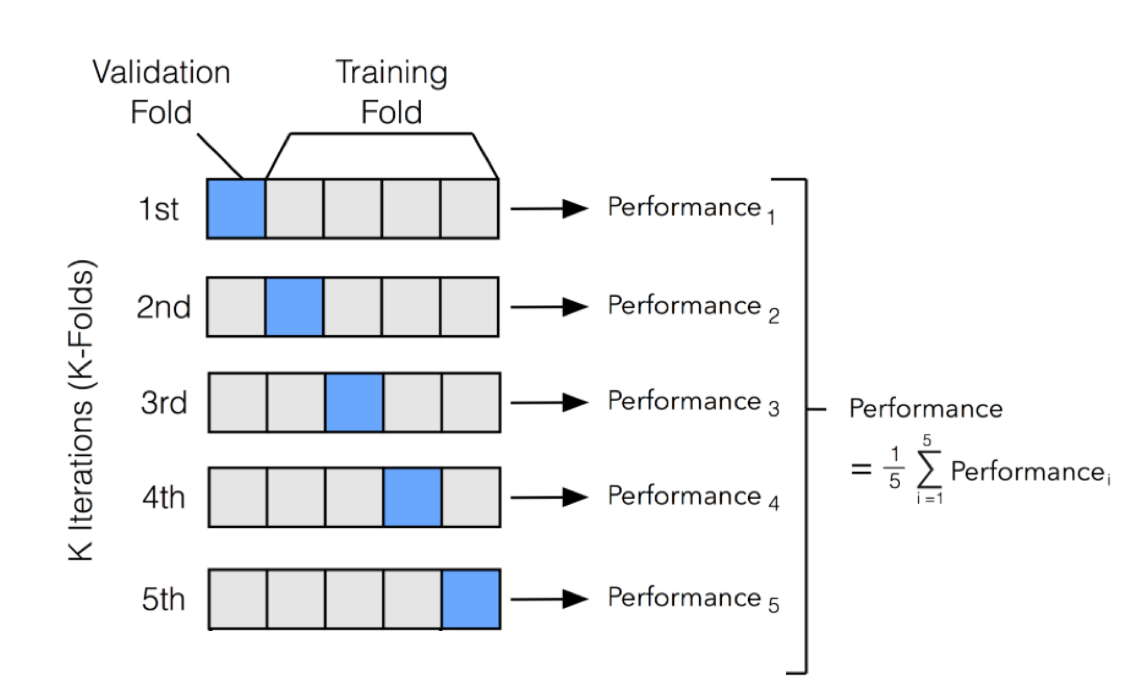
\includegraphics[width=0.7\textwidth]{kfold.png}
\caption{Esquema da validação cruzada com $k=5$: em cada rodada, uma fatia diferente é usada como conjunto de validação, e as demais como treino. Fonte: adaptado de Nishad (2023).}
\label{fig:kfold}
\end{center}
\end{figure}

%%%%%%%%%%%%%%%%%%%%%%%%%%%%%%%%%   RESULTADOS   %%%%%%%%%%%%%%%%%%%%%%%%%%%%%%%%%%%%%%%%%%%%%%%%%

\subsection{Resultados experimentais}

Foram realizados \textbf{sete experimentos} sucessivos, organizados em três blocos. O primeiro (Experimentos 1--3) varia o conjunto de \textit{features} mantendo a divisão treino/teste em 80\%/20\%. O segundo (Experimentos 4--6) investiga o impacto da \textit{feature} \texttt{kmeans\_centroid\_dist} e a sensibilidade ao tamanho do conjunto de treino. O Experimento 7 avalia a generalização da \textit{pipeline} em curvas exclusivamente reais. A Tabela~\ref{tab:resumo_exp} apresenta o melhor desempenho obtido em cada configuração.

\begin{table}[!h]
\centering
\caption{Resumo do melhor desempenho por experimento (no conjunto de teste).}
\label{tab:resumo_exp}
{\small
\begin{tabular}{clccc}
\toprule
\textbf{Exp.} & \textbf{Configuração} & \textbf{Melhor F1} & \textbf{AUC-ROC} & \textbf{Modelo líder} \\
\midrule
1 & 28 \textit{features}, \textit{split} 80/20  & 0,9937 & 0,9997 & Random Forest \\
2 & 14 \textit{features}, \textit{split} 80/20  & 0,9906 & 0,9996 & CatBoost \\
3 & 13 \textit{features}, \textit{split} 80/20  & 0,9905 & 0,9998 & Random Forest \\
4 & 12 \textit{features} (sem K-Means)          & 0,9906 & 0,9998 & Random Forest \\
5 & 11 \textit{features} (ablação combinada)    & 0,9906 & 0,9995 & XGBoost \\
6 & 11 \textit{features}, \textit{split} 65/35  & 0,9906 & 0,9995 & XGBoost \\
7 & 11 \textit{features}, teste só em reais     & 0,9821 & 0,9968 & XGBoost \\
\bottomrule
\end{tabular}
}
\end{table}

A Figura~\ref{fig:roc} apresenta as curvas ROC dos quatro modelos no Experimento 5 (configuração final, 11 \textit{features}). Todos os modelos exibem AUC-ROC $\geq 0{,}99$, com curvas fortemente deslocadas em direção ao canto superior esquerdo, indicando excelente capacidade de separação das classes.

\begin{figure}[!h]
\begin{center}
    
\includegraphics[width=0.7\textwidth]{roc_curves.png}
\caption{Curvas ROC dos quatro classificadores no Experimento 5 (11 \textit{features}, \textit{split} 80/20). Todos os modelos atingem AUC-ROC superior a 0,999.}
\label{fig:roc}
\end{center}
\end{figure}

\begin{figure}[!h]
\begin{center}
    
\includegraphics[width=0.85\textwidth]{confusion_matrices.png}
\caption{Matrizes de confusão dos quatro modelos no Experimento 5. Os erros são tipicamente unitários, distribuídos entre falsos positivos e falsos negativos de forma equilibrada.}
\label{fig:cm}
\end{center}
\end{figure}

\subsection{Estudo de ablação: a \textit{feature} K-Means}

A \textit{feature} \texttt{kmeans\_centroid\_dist} -- distância entre os dois centróides obtidos pela aplicação do K-Means com $K=2$ ao fluxo suavizado -- aparecia consistentemente como a mais importante nos modelos baseados em árvore, chegando a 63\% de importância no XGBoost. A pergunta natural era: essa importância reflete contribuição insubstituível ou apenas a oferta de um \textit{split} eficiente?

A comparação entre os Experimentos 3 (com K-Means) e 4 (sem K-Means) responde à questão: a remoção da \textit{feature} causa degradação inferior a 0,3 ponto percentual em F1 (Tabela~\ref{tab:resumo_exp}). Esse resultado tem implicação metodológica direta: \textbf{importância atribuída por algoritmos de árvore não é sinônimo de insubstituibilidade}. \textit{Features} colineares podem redistribuir a capacidade preditiva quando uma delas é removida. A Figura~\ref{fig:fi_rf} mostra a distribuição de importâncias do Random Forest no Experimento 5 (já sem o K-Means), com as métricas observacionais (\texttt{Occ\_depth}, \texttt{Occ\_SNR\_dip}, \texttt{Occ\_chi2\_ratio}) absorvendo a função discriminativa.

\begin{figure}[!h]
\begin{center}
    
\includegraphics[width=0.75\textwidth]{feature_importance_random_forest.png}
\caption{Importância das \textit{features} no Random Forest -- Experimento 5 (11 \textit{features}). As métricas observacionais (profundidade, SNR e razão $\chi^2$) lideram, mostrando que a remoção do K-Means não comprometeu a capacidade do modelo.}
\label{fig:fi_rf}
\end{center}
\end{figure}

\subsection{Verificação em curvas de baixo SNR}

Como verificação complementar, as 67 curvas do banco com $\mathrm{Occ\_SNR\_dip} < 3$ -- as mais ruidosas do conjunto -- foram submetidas aos modelos treinados. Todos os modelos baseados em árvore (Random Forest, XGBoost, CatBoost) classificaram corretamente 67 de 67 como positivas; a Regressão Logística acertou 66 de 67. Embora essas curvas tenham participado do treinamento e o teste não inclua negativos genuínos de baixo SNR, o resultado indica que os modelos não rejeitam sistematicamente eventos ruidosos -- condição necessária (embora não suficiente) para aplicabilidade em cenários de baixa relação sinal-ruído. Um teste rigoroso em conjunto difícil curado está previsto em trabalhos futuros.

\subsection{Dificuldades encontradas e suas soluções}

\textbf{Desbalanceamento residual e validade do simulador.} O \textit{dataset} final equilibra as classes (802 positivas vs.\ 891 negativas), mas a maioria das negativas é sintética ou obtida por recorte. O Experimento 7, no qual o teste é restrito a curvas exclusivamente reais, mostra queda apenas marginal de desempenho (F1 cai de 0,9906 para 0,9821), sugerindo que o simulador físico produz curvas suficientemente fiéis para treinamento. Ainda assim, a generalização para um cenário puramente observacional permanece como limitação reconhecida.

\textbf{Predominância de curvas com ocultações bem definidas.} O elevado desempenho dos modelos reflete, em parte, o fato de que a maioria das curvas no \textit{dataset} apresenta ocultações com alto SNR e queda pronunciada. Para curvas marginais (baixo SNR, eventos rasantes), a tarefa é substancialmente mais difícil e o desempenho real ainda não foi avaliado sistematicamente. A construção de um subconjunto de teste exclusivamente difícil é uma das principais direções de trabalho futuro.

\textbf{Necessidade de coronagrafia digital em alguns casos.} Durante a inserção das curvas do Grupo do Rio, observou-se que a fotometria de Umbriel exigia tratamento especial devido ao brilho intenso de Urano, motivando a aplicação de coronagrafia digital previamente à fotometria diferencial \citep{Assafin2023}. Esse procedimento foi feito no nível da redução fotométrica, anterior à \textit{pipeline} aqui apresentada.

%%%%%%%%%%%%%%%%%%%%%%%%%%%%%%%%%   PRÓXIMAS ETAPAS   %%%%%%%%%%%%%%%%%%%%%%%%%%%%%%%%%%%%%%%%%

\section{\sc Proposta para próximas etapas}

Com a \textit{pipeline} consolidada e os resultados experimentais reportados na dissertação, as próximas etapas concentram-se na finalização da escrita, na incorporação de revisões do orientador e na preparação para a defesa.

\subsection{Atividades acadêmicas previstas para o próximo período}

\begin{itemize}
    \item \textbf{Finalização da dissertação:} incorporação das revisões do orientador (já em andamento), revisão final dos capítulos 2 a 6 e do resumo, atualização da bibliografia.
    \item \textbf{Defesa:} prevista para o segundo semestre de 2026.
    \item \textbf{Submissão de artigo:} preparar versão condensada da metodologia e dos resultados para submissão à \textit{Astronomy \& Astrophysics} ou \textit{Monthly Notices of the Royal Astronomical Society}, com foco no resultado de ablação e na metodologia interpretável.
    \item \textbf{Aplicação a campanhas específicas:} validar a \textit{pipeline} em dados de campanhas observacionais de objetos como Quaoar \citep{Quaoar2023}, em cenário real de uso integrado ao SORA.
\end{itemize}

\subsection{Direções de pesquisa futura}

Embora além do escopo do mestrado, três direções identificadas durante o trabalho merecem registro como continuação natural:

\begin{itemize}
    \item \textbf{Detecção em regime de baixo S/N:} construir um subconjunto de teste composto exclusivamente por curvas difíceis (baixo SNR, ocultações rasantes, eventos com poucos pontos no \textit{dip}), para avaliar o desempenho da \textit{pipeline} nas condições em que a triagem automática é de fato necessária.

    \item \textbf{Classificação multi-classe:} estender a formulação binária para distinguir o tipo de evento (corpo sólido, assinatura atmosférica, anel, padrão de Fresnel), exigindo \textit{features} adicionais (e.g., simetria do perfil, presença de quedas secundárias) e \textit{dataset} curado por categoria.

    \item \textbf{Extração automática de parâmetros físicos:} usar os modelos não apenas para classificar, mas para estimar grandezas físicas (instantes de imersão e emersão, diâmetro projetado, escala de Fresnel efetiva), complementando a saída do SORA em campanhas com grande volume de dados.
\end{itemize}

%%%%%%%%%%%%%%%%%%%%%%%%%%%%%%%%%%%%%%%%%%%%%%%%%%%%%%%%%%%%%%%%%%%%%%%%%%%%%%%%%%%%%
%%%%%%%                     Bibliografia                                  %%%%%%%%%
%%%%%%%%%%%%%%%%%%%%%%%%%%%%%%%%%%%%%%%%%%%%%%%%%%%%%%%%%%%%%%%%%%%%%%%%%%%%%%%%%%%%%
\newpage

\bibliography{ref}
\bibliographystyle{apalike}

\end{document}
